% Latex template: mahmoud.s.fahmy@students.kasralainy.edu.eg
% For more details: https://www.sharelatex.com/learn/Beamer

\documentclass[aspectratio=169]{beamer}            % Document class

\usepackage[portuguese]{babel}          % Set language
\usepackage[utf8x]{inputenc}            % Set encoding
\usepackage{courier}
\mode<presentation> {                   % Set options
  \usetheme{default}                    % Set theme
  \usecolortheme{default}               % Set colors
  \usefonttheme{default}                % Set font theme
  \setbeamertemplate{caption}[numbered]	% Set caption to be numbered
}

\setbeamertemplate{navigation symbols}{}
\setbeamertemplate{footline}[frame number]
\setbeamercovered{transparent}

\newcommand\Wider[2][3em]{%
\makebox[\linewidth][c]{%
  \begin{minipage}{\dimexpr\textwidth+#1\relax}
  \raggedright#2
  \end{minipage}%
  }%
}

% Uncomment this to have the outline at the beginning of each section highlighted.
%\AtBeginSection[]
%{
%  \begin{frame}{Outline}
%    \tableofcontents[currentsection]
%  \end{frame}
%}

\usepackage{graphicx}                   % For including figures
\usepackage{booktabs}                   % For table rules
\usepackage{hyperref}                   % For cross-referencing
\usepackage{caption}
\usepackage{siunitx}% Allows more control over captions in figs and tables


\title{Revisão de Atividades da FAC}	% Presentation title
%\author{Author One}					% Presentation author
\institute{LNLS.DAC.FAC}				% Author affiliation
\date{2024-07-12 -- 2024-08-23}			% Today's date


% Machine studies in the period
% =============================

% 2024-07-16-SI_60hz_ff_orbit
% 2024-07-18-SI_bpm02C1_1_oscillations
% 2024-07-22-AS_machine_characterization_screens_images
% 2024-07-22-SI_acquisition_ORION_concrete
% 2024-07-28-AS_machine-shutdown



\begin{document}

\begin{frame}
  \titlepage
  \href{https://github.com/lnls-fac/doc-review-dac-fac}{\beamergotobutton{Link para o repo github desta apresentação: https://github.com/lnls-fac/doc-review-dac-fac}}
  \href{https://www.overleaf.com/read/sbdjxtzfchrm}{\beamergotobutton{Link para o projeto overleaf destas notas}}
\end{frame}

\begin{frame}{Outline}
  \tableofcontents
\end{frame}

\section{Caracterização da Máquina - Pré-parada}

% 2024-07-22-AS_machine_characterization_screens_images


\begin{frame}{Caracterização da Máquina - Pré-parada}

{\footnotesize
% \vspace{-0.3cm}
\begin{itemize}
    % \setlength\itemsep{1em}
    \item estudo dia 2024-07-22
\end{itemize}
}
% % \vspace{-0.2cm}
% \begin{figure}[ht]
%     \begin{minipage}[b]{0.4\linewidth}
%         \centering
%         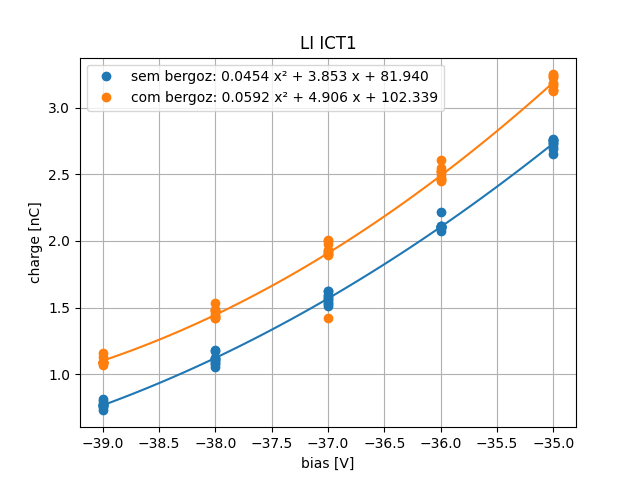
\includegraphics[width=\textwidth]{2024-07-12/figures/li-ict1.png}
%         \caption{Calibration of LI ICT1.}
%         \label{fig:a}
%     \end{minipage}
%     \hspace{0.2cm}
%     \begin{minipage}[b]{0.4\linewidth}
%         \centering
%         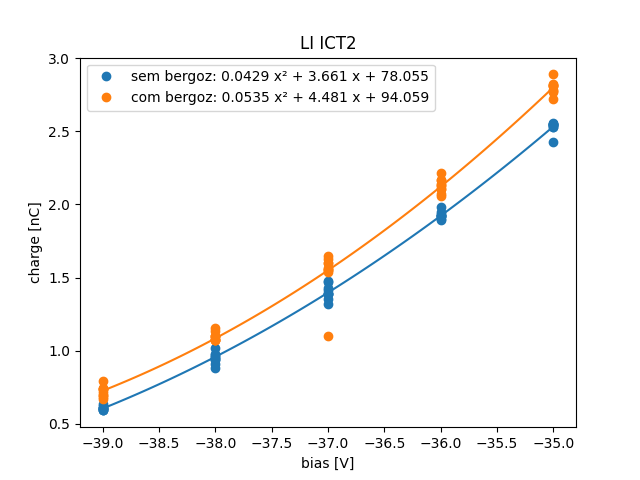
\includegraphics[width=\textwidth]{2024-07-12/figures/li-ict2.png}
%         \caption{Calibration of LI ICT2.}
%         \label{fig:b}
%     \end{minipage}
% \end{figure}
\end{frame}

\section{FF de órbita para perturbação em 60 Hz}

% 2024-07-16-SI_60hz_ff_orbit

\begin{frame}{FF de órbita para perturbação em 60 Hz}

{\footnotesize
\begin{itemize}
    \setlength\itemsep{0.5em}
    \item estudos em 2024-05-14 e 2024-07-01 \href{https://ais-eng-srv-ta.cnpem.br/Olog/index.html\#22801\_4}{\beamergotobutton{Olog \#22801\_4}}
    \item no primeiro estudo, apenas caracterização do FF, sem SOFB.
    \item no segundo estudo testamos nova versão do SOFB com as corretoras no modo \ot{RmpWfm} e agindo no \it{WfmOffsetKick}.
\end{itemize}
}
\vspace{-0.2cm}
\centering
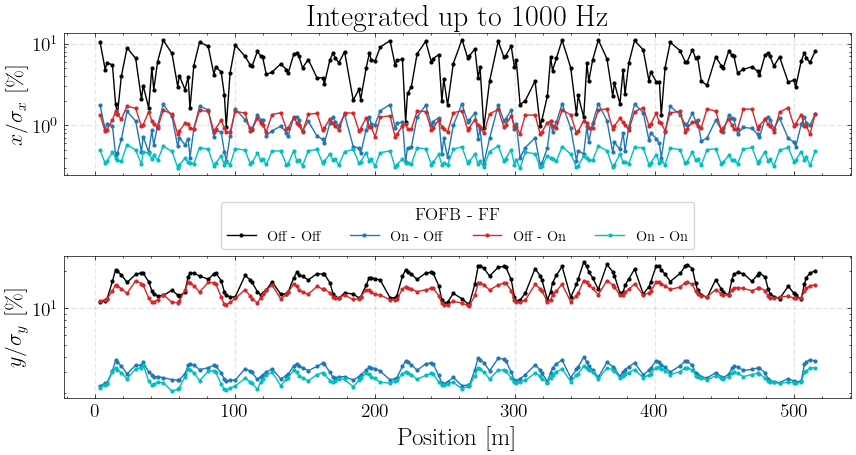
\includegraphics[width=0.7\linewidth]{2024-07-12/figures/integrated_distortion_up_to_1000Hz_run2.png}
\end{frame}

\section{Especificação da 3HC}


\begin{frame}{Especificação da 3HC}

{\footnotesize
\begin{itemize}
    \setlength\itemsep{0.5em}
    \item Item1
\end{itemize}
}
\vspace{-0.2cm}
% \centering
% 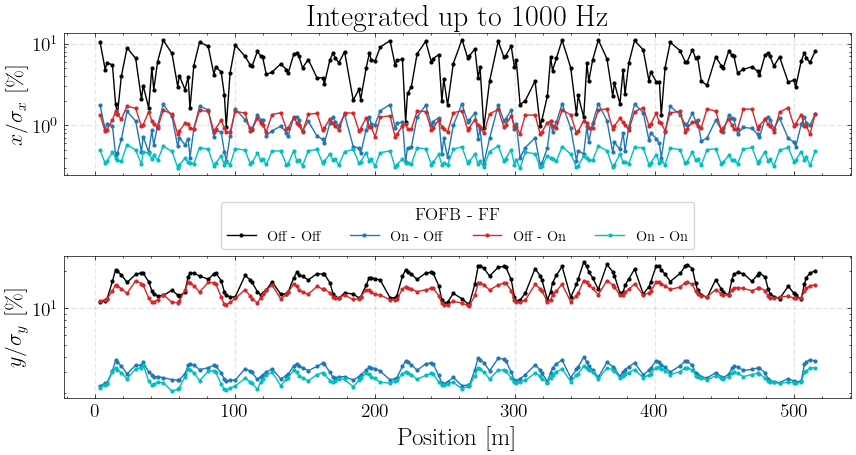
\includegraphics[width=0.7\linewidth]{2024-07-12/figures/integrated_distortion_up_to_1000Hz_run2.png}
\end{frame}

\section{Reconstrução de densidade no espaço de fase}


\begin{frame}{Reconstrução de densidade no espaço de fase}

{\footnotesize
\begin{itemize}
    \setlength\itemsep{0.5em}
    \item Item1
\end{itemize}
}
\vspace{-0.2cm}
% \centering
% 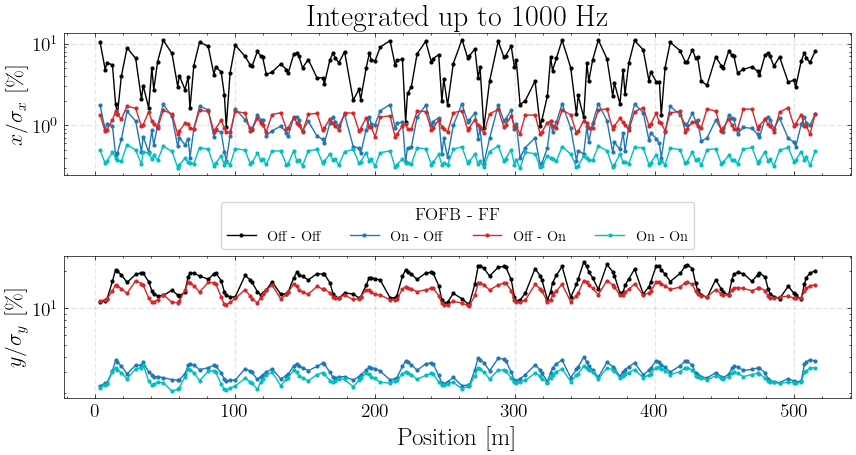
\includegraphics[width=0.7\linewidth]{2024-07-12/figures/integrated_distortion_up_to_1000Hz_run2.png}
\end{frame}

\section{Curvas de excitação dos trims de quadrupolos}


\begin{frame}{Curvas de excitação dos trims de quadrupolos}

{\footnotesize
\begin{itemize}
    \item Item1
\end{itemize}
}
\vspace{-0.2cm}
% \centering
% 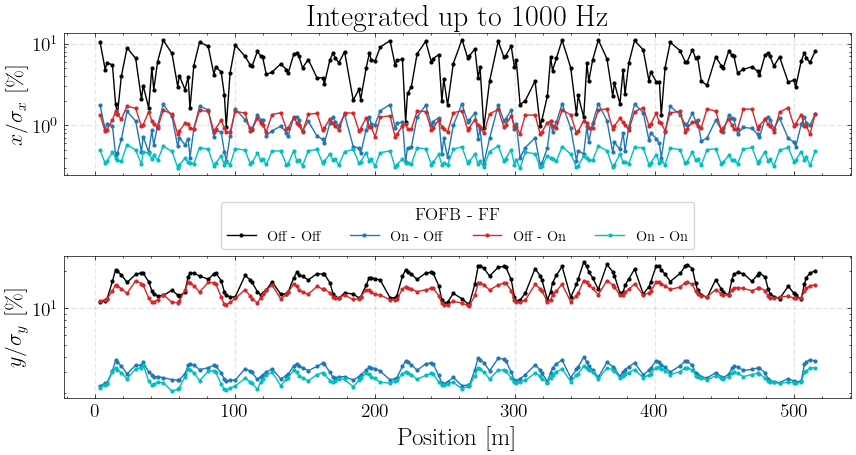
\includegraphics[width=0.7\linewidth]{2024-07-12/figures/integrated_distortion_up_to_1000Hz_run2.png}
\end{frame}

\section{Reorganização dos Sensores de Temperatura}


\begin{frame}{Reorganização dos Sensores de Temperatura}

{\footnotesize
\begin{itemize}
    \item Item1
\end{itemize}
}
\vspace{-0.2cm}
% \centering
% 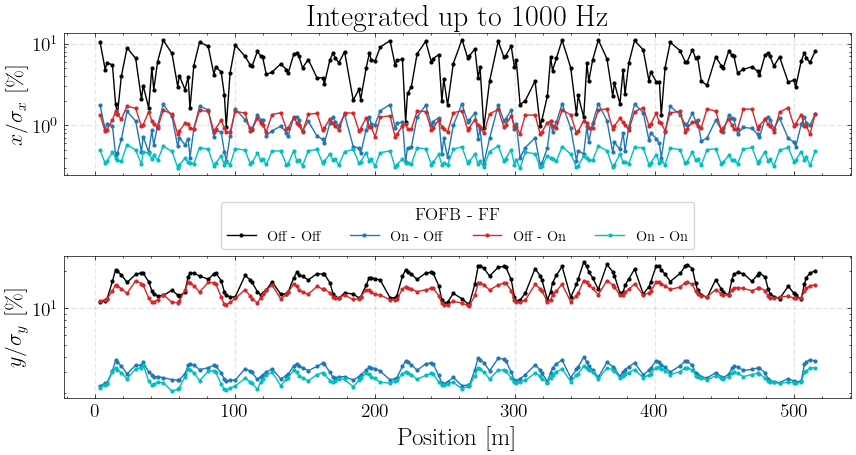
\includegraphics[width=0.7\linewidth]{2024-07-12/figures/integrated_distortion_up_to_1000Hz_run2.png}
\end{frame}

\section{Aprimoramentos dos códigos da FAC}


\begin{frame}{Aprimoramentos dos códigos da FAC}

{\footnotesize
\begin{itemize}
    \item Item1
\end{itemize}
}
\vspace{-0.2cm}
% \centering
% 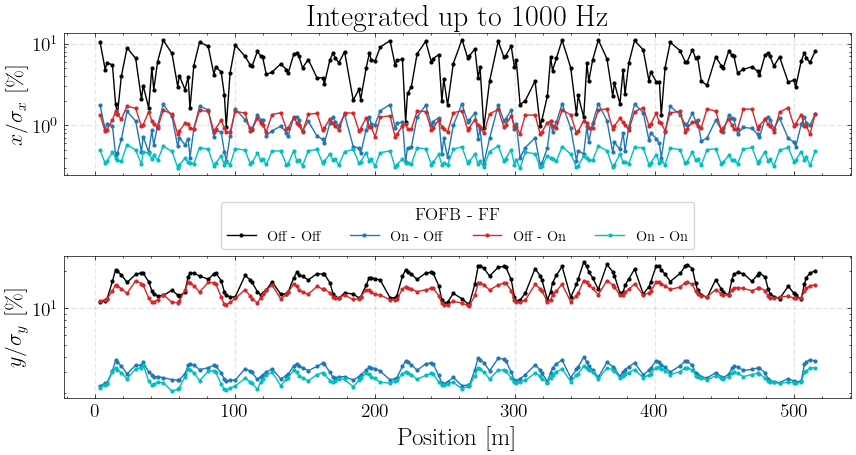
\includegraphics[width=0.7\linewidth]{2024-07-12/figures/integrated_distortion_up_to_1000Hz_run2.png}
\end{frame}

\end{document}
